\documentclass{beamer}
\usetheme{CambridgeUS}
\setbeamercovered{transparent}
%\usetheme{Hannover}

%\usetheme{Copenhagen}
\usepackage{graphicx}
\usepackage[utf8]{inputenc}
\usepackage[english]{babel}
\usepackage{calc}
\usepackage{amsmath}
\DeclareMathAlphabet{\mathonebb}{U}{bbold}{m}{n}
\usepackage{verbatimbox}
\usepackage{verbatim}
\usepackage{moreverb}
\usepackage{eurosym}
\usepackage{verbatim}      
\usepackage{amsmath, amsthm}                             
 
\usepackage{latexsym}                               
\usepackage{amssymb}
\usepackage{tabularx}
\usepackage{setspace}
\usepackage{listings}
\usepackage{geometry}


\usepackage{listings}
\definecolor{dkgreen}{rgb}{0,0.4,0}
\definecolor{gray}{rgb}{0.5,0.5,0.5}
\definecolor{mauve}{rgb}{0.58,0,0.82}

\usepackage[lined]{algorithm2e}
\newcommand{\algorithmicrequire}{\textbf{Input:}}
\newcommand{\algorithmicensure}{\textbf{Output:}}
\newcommand{\sign}{\text{sign}}
\newcommand{\argmin}{\text{argmin}}
\newcommand{\Cut}{\text{Cut}}
\newcommand{\Vol}{\text{Vol}}
\newcommand{\RCut}{\text{RCut}}
\newcommand{\NCut}{\text{NCut}}
\newcommand{\NCC}{\text{NCC}}
\newcommand{\RCC}{\text{RCC}}
\newcommand{\one}{\ensuremath{\mathonebb{1}}}


\usepackage{array}
\newcolumntype{L}[1]{>{\raggedright\let\newline\\\arraybackslash\hspace{0pt}}m{#1}}
\newcolumntype{C}[1]{>{\centering\let\newline\\\arraybackslash\hspace{0pt}}m{#1}}
\newcolumntype{R}[1]{>{\raggedleft\let\newline\\\arraybackslash\hspace{0pt}}m{#1}}

\usepackage{xcoffins}
\NewCoffin\tablecoffin
\NewDocumentCommand\Vcentre{m}
  {%
    \SetHorizontalCoffin\tablecoffin{#1}%
    \TypesetCoffin\tablecoffin[l,vc]%
  }


\definecolor{dkyellow}{cmyk}{0, 0, 0.2, 0}
\lstset{
  language=R,                % the language of the code
  basicstyle= \footnotesize,      % the size of the fonts that are used for the code
  numbers=left,                   % where to put the line-numbers
  numberstyle=\tiny\color{gray},  % the style that is used for the line-numbers
  stepnumber=2,                   % the step between two line-numbers. If it's 1, each line 
                                  % will be numbered
  showspaces=false,               % show spaces adding particular underscores
  showtabs=false,                 % show tabs within strings adding particular underscores
  frame=single,                   % adds a frame around the code
  rulecolor=\color{black},        % if not set, the frame-color may be changed on line-breaks within not-black text (e.g. commens (green here))
  tabsize=2,                      % sets default tabsize to 2 spaces
  captionpos=b,                   % sets the caption-position to bottom
  breaklines=true,                % sets automatic line breaking
  breakatwhitespace=false,        % sets if automatic breaks should only happen at whitespace
  keywordstyle=\color{blue},      % keyword style
  commentstyle=\color{dkgreen},   % comment style
  stringstyle=\color{mauve},       % string literal style
  backgroundcolor=\color{white},      % choose the background color. You must add \usepackage{color}
}

\usepackage{array}
\newcolumntype{L}[1]{>{\raggedright\let\newline\\\arraybackslash\hspace{0pt}}m{#1}}
\newcolumntype{C}[1]{>{\centering\let\newline\\\arraybackslash\hspace{0pt}}m{#1}}
\newcolumntype{R}[1]{>{\raggedleft\let\newline\\\arraybackslash\hspace{0pt}}m{#1}}

\usepackage{blkarray}% http://ctan.org/pkg/blkarray
\newcommand{\matindex}[1]{\mbox{\scriptsize#1}}% Matrix index

\title{Cell cycle analysis by live imaging}

\author{Peter Naylor}

\date{Internship defense}

\AtBeginSection[]
{
  \begin{frame}<beamer>{Sommaire}
    \tableofcontents[currentsection,currentsubsection]
  \end{frame}
}

\begin{document}

\begin{frame}
  \titlepage
\end{frame}

\begin{frame}{Introduction}

Interest: Understanding the human genome.

\begin{columns}[T] % align columns
\begin{column}{.50\textwidth}

\begin{itemize}
\item A gene produces a protein.
\item Cell cycle regulated by proteins.
\item Interested in the non-mitotic phases.
\end{itemize}

Contents:
\begin{enumerate}
\item Biological context
\item Classification of cell cycle phases
\item Application to a large scale screening data set
\item Transfer learning
\end{enumerate}

\end{column}%

\hfill%
\begin{column}{.30\textwidth}
\begin{figure}[!ht]
\centering
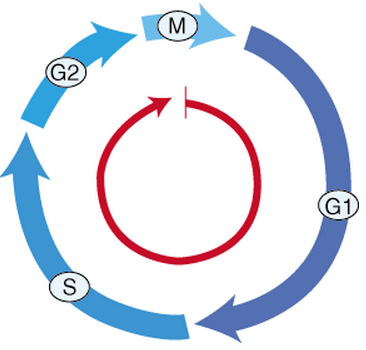
\includegraphics[width=\textwidth]{Images/somaticcellcycle3.png}
\caption{Cell cycle}
\label{cellcycle}
\end{figure}
\end{column}%
\end{columns}

\end{frame}





\begin{frame}{How to infer protein function}
Two existing technics, which are complementary:
\begin{itemize}
\item Making hypothesis on their function based on their location in the cell \\ 
\textit{Using flurorescent markers, protein track within the cell} 
\item We make an experience where a certain protein is absent from the cell \\ 
\textit{Characterising cell aspects and its evolution w.r.t time} \\ 
 $\rightarrow$ For example, if the cell cycle is disrupted.
\end{itemize}
\end{frame}


\begin{frame}{MitoCheck Project}
\begin{itemize}
\item<1> \begin{center}
{\small \textit{Published genome wide dataset of time-resolved records of cellular phenotype responses to loss-of-function experiments.} }\\ 
\end{center}

\item<2> MitoCheck database: 
\begin{itemize}
\item Loss-of-function screening
\item Genome-wide RNAi screening
\item Live imaging
\item Chromosome marker (H2B)
\end{itemize} 

%%%Currently working on MitoCheck like database.\\
%%%Live imaging with H2B markers but labeled by PCNA-marker. \\
%%%\pause 
%%%Extensions of my work: Applying it to the MitoCheck database. \\ 
\textbf{Goal:} Understanding what genes play a role and where in the non-mitotic phases. \\
\textbf{Difficulty:} \begin{itemize}
    \item Fluorescent marker informative about the mitotic-phases.
    \item No ground truth.
    \end{itemize}
\end{itemize}
\end{frame}

\begin{frame}{The raw data}
\begin{columns}[T] % align columns
\begin{column}{.40\textwidth}
\begin{footnotesize}
\begin{figure}[!ht]
\centering
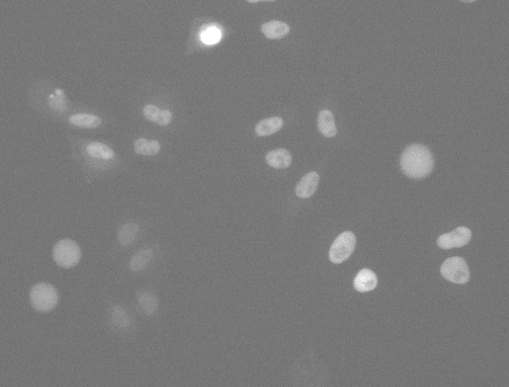
\includegraphics[width=0.50\textwidth]{Images/PCNA.png}
\caption{Data acquired by Michael Olma with the \texttt{PCNA} marker}
\label{PCNA_michael_olma}
\end{figure}


\begin{itemize}
\item Data set that helps us label the data.
\item HeLa cells stably expressing \texttt{PCNA} marker which is informative about the non-mitotic phases.
\end{itemize}
\end{footnotesize}

\end{column}%

\hfill%

\begin{column}{.56\textwidth}
\begin{footnotesize}
\begin{figure}[!ht]
\centering
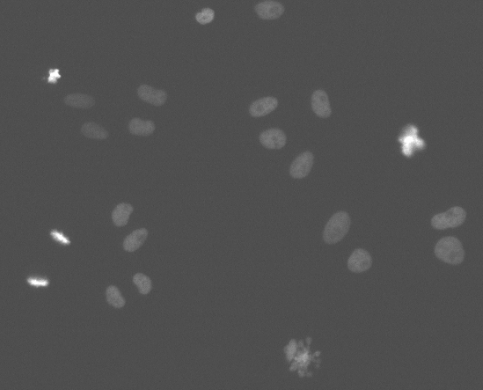
\includegraphics[width=0.38\textwidth]{Images/H2B.png}
\caption{Data acquired by Michael Olma with the \texttt{H2B} marker}
\label{H2B}
\end{figure}


\begin{itemize}
\item Data set from which we extract features for training purposes. 
\item Looking for paterns that help differenciate non-mitotic phases.
\item HeLa cells stably expressing \texttt{H2B} marker, informative about the mitotic phases.
\end{itemize}
\end{footnotesize}

\end{column}%

\end{columns}


\end{frame}

\iffalse

\begin{frame}{The raw data}
\begin{figure}[!ht]
\centering
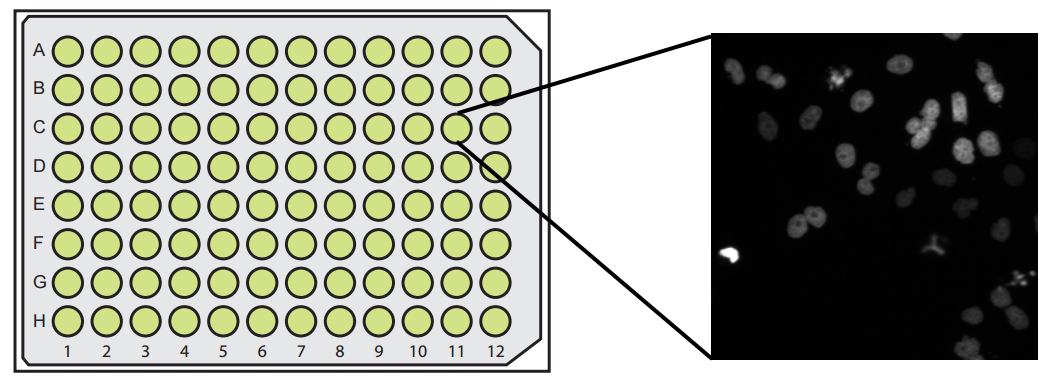
\includegraphics[width=0.60\textwidth]{Images/plate_well.png}
\caption{MitoCheck dataset}
\label{Mitocheck_well}
\end{figure}

\begin{itemize}
\item HeLa cells stably expressing \texttt{H2B} marker, informative about the mitotic phases.
\item Goal: detect the non-mitotic phases.
%%\item Difficulties: The extracted features don't follow the same exact distributions.
\end{itemize}
\end{frame}

\fi

\begin{frame}{Extracting the data}

Using \textit{CellCognition}:
\begin{figure}[!ht]
\centering
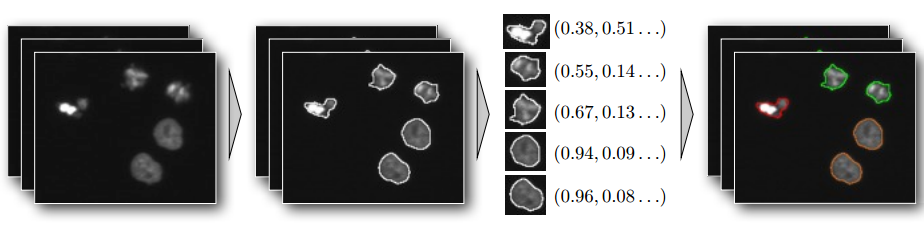
\includegraphics[width=\textwidth]{Images/features_extract.png}
\caption{\textit{CellCognition} steps for feature extraction}
\label{extract}
\end{figure}

We can reach an accuracy of 69\%. \\
Live imaging $\longrightarrow$ taking time into account: 2 methods.
\end{frame}

\iffalse

\begin{frame}{Nested Cross validation}
\begin{figure}[!ht]
\centering
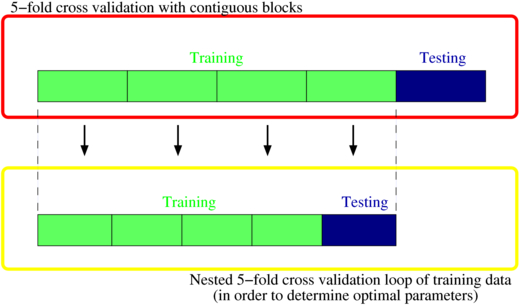
\includegraphics[width=0.6\textwidth]{Images/nest_cv.jpg}
\caption{Nested Cross validation}
\label{NestedCV}
\end{figure}
Upper biaises the accuracy! \\
Without the nested cross validation: 71\%. \\
With the nested cross validation: 69\%.
\end{frame}

\fi

\begin{frame}{Normalizing the data}
Same idea as in Panel data, try to get ride of the cell-specific, time-invariant effects. (Size, intensity...)\\
%%Using Alice's work on cell trajectory.
Using the full cell trajectories.

\begin{figure}[!ht]
\centering
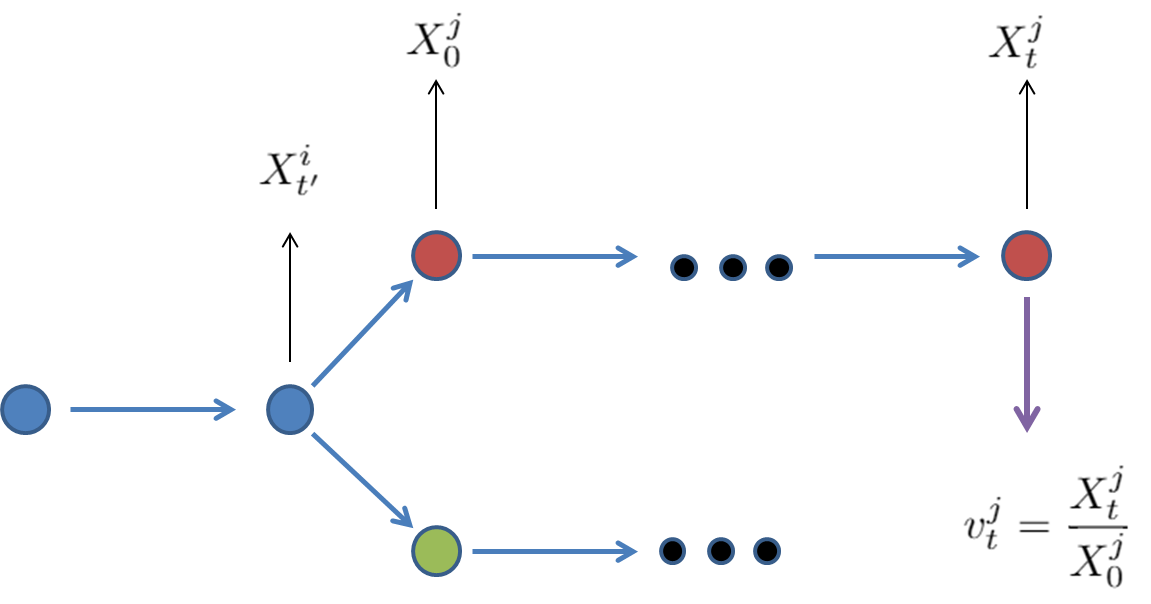
\includegraphics[width=0.6\textwidth]{Images/test1.png}
\caption{Normalisation of the data}
\label{normalization}
\end{figure}

Increases the accuracy to 78\%. (Very little signal from \textit{G2}.)
\end{frame}

\iffalse

\begin{frame}{Normalizing the data (2/2)}
\begin{itemize}
\item Increases the accuracy to 78\%.
\item Biais and data size reduces by half, only scales to cell trajectories initially starting with a mitosis. We drop to 472 annotated cells.
\item We have very little signal for phase \textit{G2}. 
\end{itemize}
\end{frame}

\fi

\iffalse

Confusion matrix for the \textbf{un}normalized data:

\[
  \begin{blockarray}{cccc}
 \multicolumn{3}{c}{\textit{Grounds Truth}} & \\
    \matindex{\textit{G1}} & \matindex{\textit{S}} &\matindex{\textit{G2}} & \\
    \begin{block}{(ccc)c}
   269 & 65 & 10 & \matindex{\textit{G1}} \\
   107 & 443 & 142 & \matindex{\textit{S}} \\
   2   & 39 & 83 & \matindex{\textit{G2}}  \\
    \end{block}
      &   &    &  \\
      \multicolumn{3}{c}{\underline{Confusion Matrix}} & 
  \end{blockarray}
  \longrightarrow
  \begin{blockarray}{cccc}
 \multicolumn{4}{c}{}  \\
    \matindex{\textit{G1}} & \matindex{\textit{S}} &\matindex{\textit{G2}} & \\
    \begin{block}{(ccc)c}
   0.712 & 0.119 & 0.043 & \matindex{\textit{G1}} \\
   0.283 & 0.810 & 0.604 & \matindex{\textit{S}}  \\
   0.005 & 0.071 & 0.353 & \matindex{\textit{G2}} \\
    \end{block}
      &   &    &  \\
      \multicolumn{3}{c}{\underline{Emission matrix}} &
  \end{blockarray}
\]

\fi

\iffalse

\begin{frame}{Hidden Markov Model}
To more strongly take into account time dependencies, we use a Hidden State Markov model. \\
An observation sequence: tracking and first model prediction for one cell in each of the frame in which he appears. 
\begin{figure}[!ht]
\centering
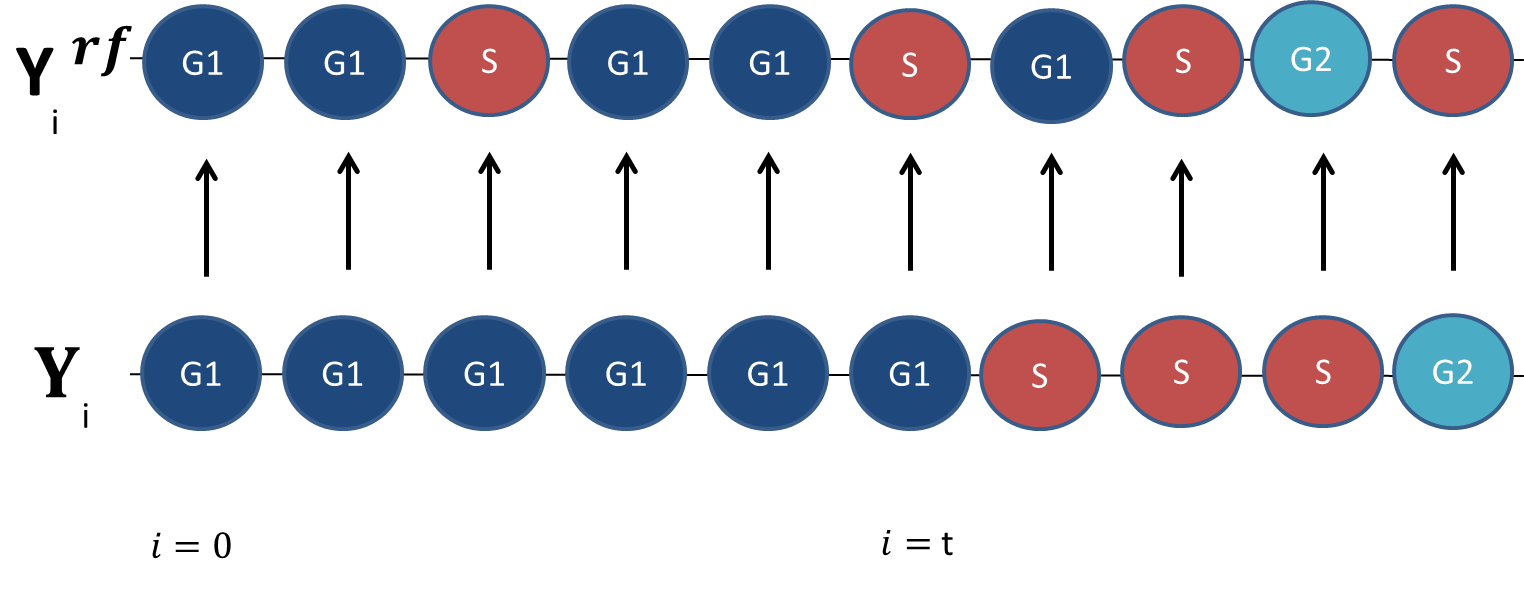
\includegraphics[width=0.8\textwidth]{Images/HMM.png}
\caption{Correcting a trajectory with the hidden markov chain}
\label{trajectory}
\textit{$Y^{rf}_i$ is the prediction of the cell at a certain frame $i$, $Y_i$ in its true state}
\end{figure}

\end{frame}

\fi

\begin{frame}{Hidden Markov Model}

\begin{columns}[T] % align columns
\begin{column}{.48\textwidth}
\begin{figure}[!ht]
\centering
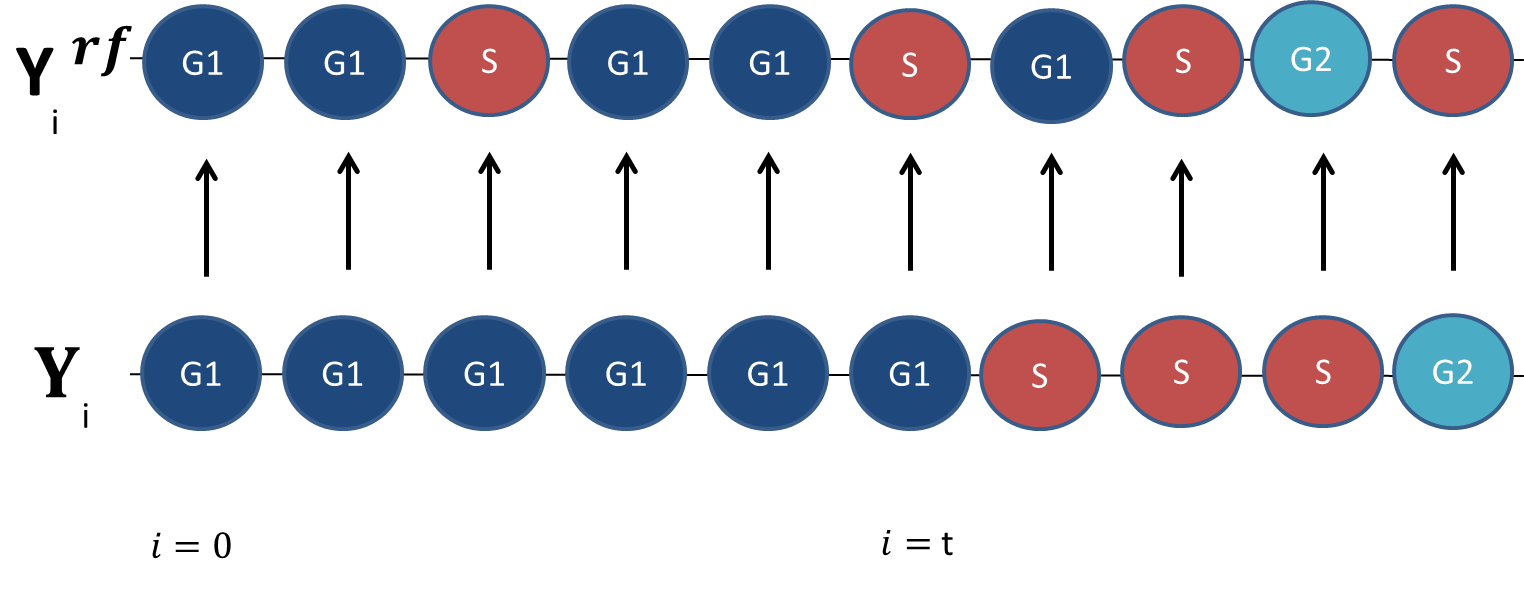
\includegraphics[width=0.95\textwidth]{Images/HMM.png}
%%\caption{Correcting a trajectory with the hidden markov chain}
\label{trajectory}
%%\textit{$Y^{rf}_i$ is the prediction of the cell at a certain frame $i$, $Y_i$ in its true state}
\end{figure}

\begin{figure}[!ht]
\centering
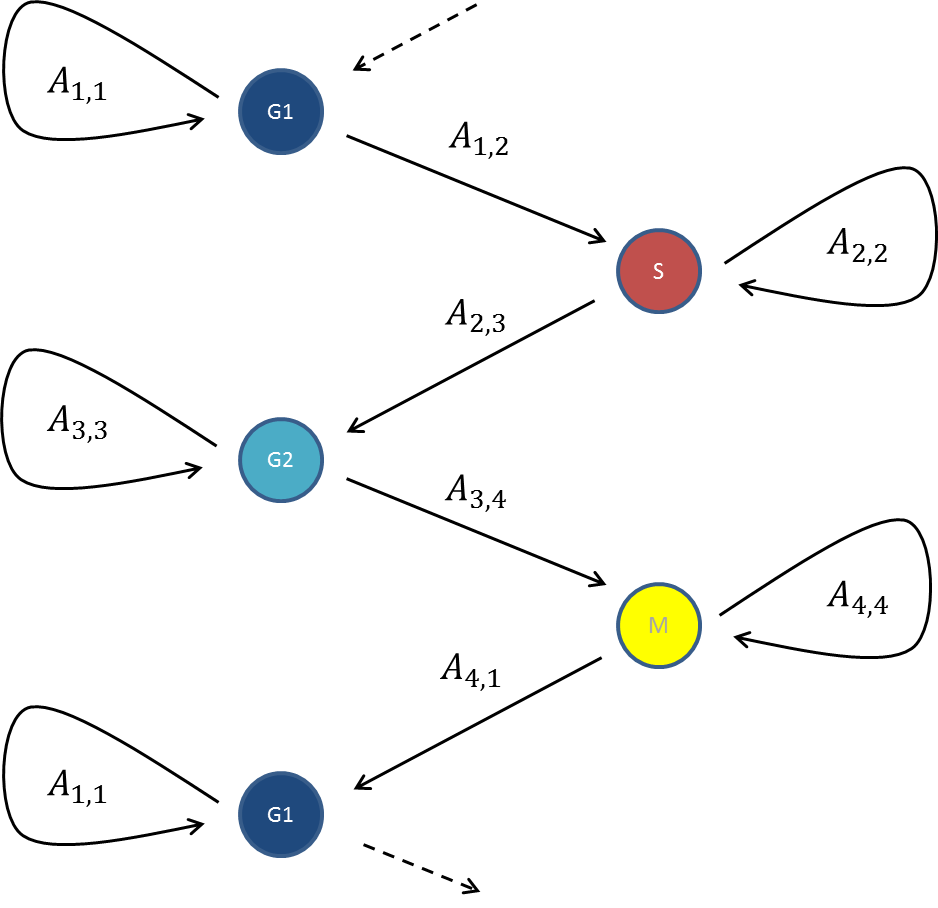
\includegraphics[width=0.6\textwidth]{Images/HMCmodel4.png}
\caption{Hidden markov model}
\label{statetransition}
\end{figure}
\end{column}%

\hfill%

\begin{column}{.48\textwidth}
\begin{itemize}
\item Strong prior on the transition matrix, we stop transition skips and returns.
\item Problem: 1st prediction is too poor. 
\item Emission probability of \textit{G2} too small.
\item We reach an accuracy of 81\%, but without predictions of class \textit{G2}.
\item If we merge state \textit{S} and state \textit{G2} we reach 94\% accuracy.
\end{itemize}
\end{column}%
\end{columns}
\end{frame}

\iffalse

\begin{frame}{Results}
\begin{figure}[!ht]
\centering
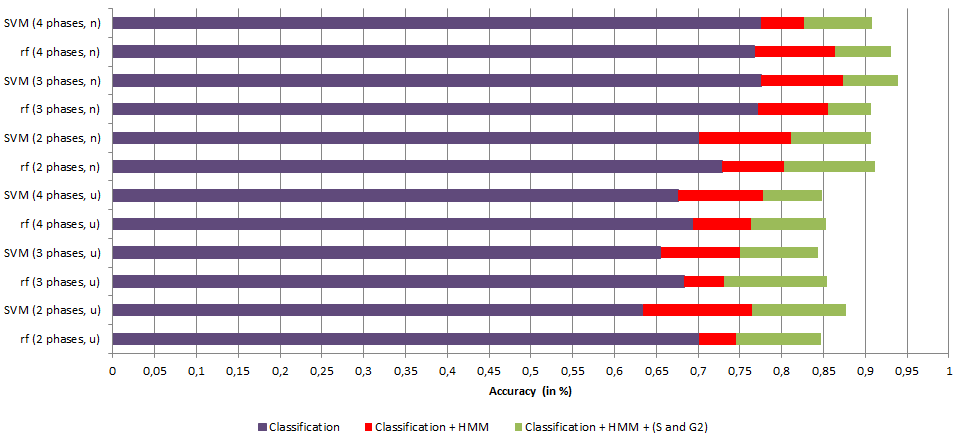
\includegraphics[width=\textwidth]{Images/Accuracy_models.png}
\caption{Accuracy results for different models where the number of folds was 10.}
\label{Results_Acc}
\end{figure}
\end{frame}

\fi

\begin{frame}{Final Classifier}
\begin{figure}[!ht]
\centering
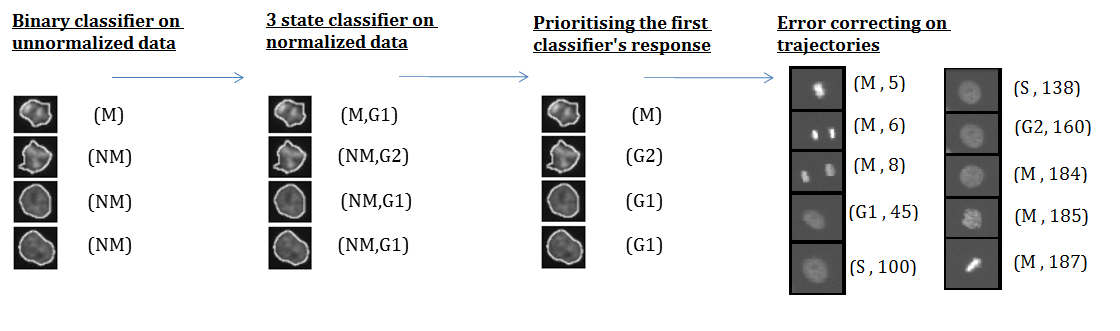
\includegraphics[width=\textwidth]{Images/Final_classif.png}
\caption{Final classifier (the error correcting model is missing).}
\label{Final_classifier}
\end{figure}
\end{frame}

\begin{frame}{Applying it to the MitoCheck data.}
\begin{table}[!ht]
\centering
\begin{tabular}{|c|c|c|c|}
  \hline
  Length of:  & Mean & Standard deviation & Number of trajectories \\
  \hline
\text{G1} & 11.76 & 6.27 & 277 \\
  \hline
\text{S}  & 5.81 & 3.64 & 194 \\
  \hline
\text{G2} & 5.19 & 4.19 & 29 \\
  \hline
\text{Cell Cycle} & 23.00 & 3.94 & 29 \\
  \hline 
\end{tabular} 
  \caption{Basic characteristics of phases length on the MitoCheck data set.}
\end{table}
\begin{itemize}
\item Out of 2408 full trajectories. Poor result.
\item Idea to improve: Tranfer Learning.
\end{itemize}
\end{frame}


\begin{frame}{Transfer learning}
\framesubtitle{Reweighting approach}

\begin{itemize}
\item One aspect of transfer learning, instance reweighting.
\item Idea, finding suitable candidates of the training set that look the most like the data we are going to predict.
\item Bayesian framework, data originates from a hidden variable. So instance $x_i$ will be reweighted by $\beta(x_i)=\frac{p(x_i|\theta)}{p(x_i|\lambda)}$.
\end{itemize}
\begin{figure}[!ht]
\centering
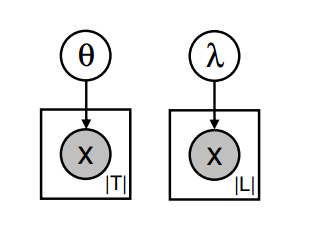
\includegraphics[width=0.3\textwidth]{Images/Method1.png}
\caption{Learning under covariate shift by estimating training
and test densities separately (image taken from \cite{pict})}
\label{fig: Method1}
\end{figure}


\end{frame}

\begin{frame}{Transfer learning}
\framesubtitle{Kernel Mean Matching}
\begin{itemize}
\item Hard to estimate multidimensionnal densities.
\item With KMM no need to estimate the densities.
\item Optimisation problem:
\end{itemize}
$$||\frac{1}{m}\underset{i=1}{\overset{m}{\sum}}\beta(x_i)\phi(x_i) - \frac{1}{m'}\underset{i=1}{\overset{m'}{\sum}}\phi(x'_i)|| = \frac{1}{m^2}\beta^T K \beta - \frac{2}{m^2} \kappa^T\beta + \text{const} $$
Where $K_{ij}=k(x_i,x_j)$ and $\kappa_i=\frac{m}{m'}\underset{j=1}{\overset{m'}{\sum}}k(x_i,x'_j)$. And: 
$$\underset{\beta}{\text{minimize}} \frac{1}{2}\beta^TK\beta-\kappa^T\beta \text{\ subject \ to } \beta_i \in [0;B] \text{\ and \ } |\underset{i=1}{\overset{m}{\sum}}\beta_i-m | \leq m\epsilon$$.

\end{frame}

\begin{frame}{Kernel Mean Matching results}

\begin{table}[!ht]
\centering
\begin{tabular}{|c|c|c|c|}
  \hline
  Length of:  & Mean & Standard deviation & Number of trajectories \\
  \hline
\text{G1} & 12 & 6.5 & 343 \\
  \hline
\text{S}  & 5.8 & 3.9 & 252 \\
  \hline
\text{G2} & 5.4 & 5.1 & 108 \\
  \hline
\text{Cell Cycle} & 23.00 & 3.8 & 78 \\
  \hline 
\end{tabular} 
  \caption{Basic characteristics of phases length on the MitoCheck data set, with transfer learning.}
\end{table}
\begin{itemize}
\item $k$ was chosen as a gaussian matrix with a hyper parameter $\sigma=1$.
The other parameters were chosen to be $\epsilon=0.9$ and $B=10$
\item Only the number of trajectories has changed. 
\end{itemize}
\end{frame}

\begin{frame}{Conclusion and futur work}

\begin{itemize}
\item It seems we can seperate phases \textit{G1} and \textit{S}. \\
If we regroup \textit{S} and \textit{G2}, we reach 93 \% of accuracy. 
\item We applied this to the MitoCheck database, poor results. We had to do transfer learning. 
\item More experiments may be conducted in order to have some ground truth. 
\item We have some for Michael Olma's data. 
\item Change the transfer learning technic, instead of instance reweighting, trying: \\
\begin{itemize}
    \item Feature representation transfer.
    \item Parameter transfer.
    \end{itemize} 
\end{itemize}

\end{frame}

\begin{frame}{Bibliographie}
\begin{thebibliography}{9}

\bibitem{ThomasNature} Held M., Schmitz M.H., Fischer B., Walter T., Neumann B., Olma M.H., Peter M., Ellenberg J. \& 
Gerlich, D.W.: \textit{CellCognition: time resolved phenotype annotation in high throughput live cell imaging.} \textbf{Nature Methods.} August 2010.


\bibitem{MitoCheck} Presentation of the MitoCheck project, \texttt{http://www.mitocheck.org/}.


\bibitem{CellCognition} The CellCognition software and presentation, \texttt{http://www.cellcognition.org/}.


\bibitem{Features} \textit{Technical Report: Feature extraction}, Walter T. January 2007. The paper was added to the annexe, in the following pages.

\bibitem{KMM} Huang, Jiayuan, et al. \textit{Correcting sample selection bias by unlabeled data.} Advances in neural information processing systems. 2006.

\bibitem{pict} Bickel, Steffen, Michael Brückner, and Tobias Scheffer. "Discriminative learning for differing training and test distributions." Proceedings of the 24th international conference on Machine learning. ACM, 2007.
\end{thebibliography}
\end{frame} 
\end{document}